\hsection{Interlude:~The Python Documentation and other Information Resources}%
\label{sec:pythonDocumentation}%
%
I~learned programming in the 1990s.
It was mainly self-taught.
I~was in seventh grade when I first saw \pgls{turboPascal}~\cite{B1992TPV7UB}, a programming language popular at that time.
I~immediately know that this is what I want to do.
My self-teaching experience was based on two pillars:
Books borrowed from friends and the really great help system of \pgls{turboPascal}.
You see, that programming language shipped with a \pgls{ide}, just like \pycharm\ is.
This \pgls{ide} was text-based, but it had lots of cool features, such as a good compiler and \pgls{debugger}.
But it also had a help system that listed every single command provided by the language.
And each command came with an example.
Sometimes I would just randomly scroll through the list, click on some command, and try out the example.
It was beautiful.
I loved it.

So that was an important part of my experience.
Which means that something similar should be available for you as you are learning \python.
Sadly, \pycharm\ cannot offer such a list of commands as good old \pgls{turboPascal} did.
Because the team behind \pycharm\ is not the team that creates and maintains \python.

Now, in the previous section, we discussed lots of functions, \pythonilIdx{sin}, \pythonilIdx{cos}, \pythonilIdx{tan}, \pythonilIdx{atan}, \pythonilIdx{exp}, \pythonilIdx{log}, \pythonilIdx{round}, \pythonilIdx{floor}, \pythonilIdx{trunc}, and~\pythonilIdx{ceil}, to name just a few.
You could read about and explore what these functions do in this book, to some degree.
As said, books were one side of the experience.
You need them to get the big picture, to understand programming paradigms, to develop an understanding of broad concepts.

But books like this one here cannot be your only source of information.
This book can only provide brief introductions into these functions from a didactic perspective.
It does not make any sense to here discuss their exact specifications and relationships to other functions in the \python\ ecosystem and neither can we exhaustively explore all the possible aspects of the \python\ language.
This leads to two questions:%
%
\begin{enumerate}%
%
\item Where do you turn to if you need to know the exact authoritative\footnote{%
\emph{Authoritative} means that the information stems from the proper standardizing organization. %
For \python, this is the \citelist{PSF:P3D}{publisher}. %
Such organizations determine the specification of functions.%
} specification of a function?%
%
\item From this book, you only learn about the functions that we \emph{do} list.
Where do you turn to if you want to do something but do not know what commands or combination of commands can be used to achieve it?%
%
\end{enumerate}%
%
\hsection{Using the Authoritative Documentation}%
\label{sec:authorativeDoc}%
%
\begin{figure}%
\begin{noglslink}%
\centering%
%
\subfloat[][%
We open a browser and visit the \citetitle{PSF:P3D}~\cite{PSF:P3D} at~\citeurl{PSF:P3D}.%
\label{fig:pythondoc01website}%
]{\tightbox{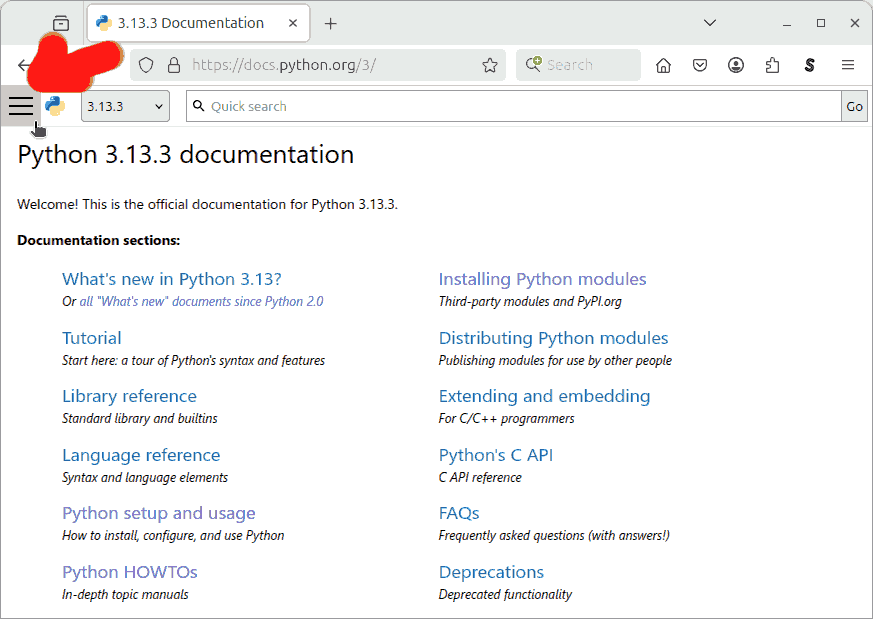
\includegraphics[width=0.47\linewidth]{\currentDir/pythondoc01website}}}%
%
\floatSep%
%
\subfloat[][%
If you click the \menu{\threeBarButton} at on the top-left corner of the website, you can get to a menu where you can change the language and, e.g., select simplified Chinese~(简体中文)~\cite{SCR1956ROTSCOPTSCCS1} if that is your preferred language.~%
(I will not do so and instead continue in English.)%
\label{fig:pythondoc02language}%
]{\tightbox{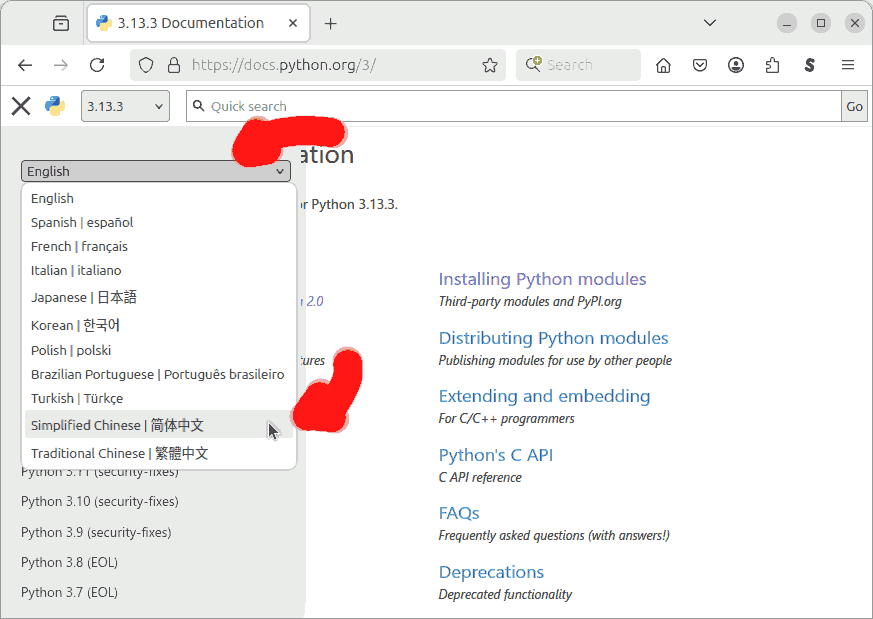
\includegraphics[width=0.47\linewidth]{\currentDir/pythondoc02language}}}%
%
\floatRowSep%
%
\subfloat[][%
We are looking for information on the \pythonilIdx{ceil} function and therefore type \pythonilIdx{ceil} into the search bar \emph{of the website} and click on~\menu{Go}.%
\label{fig:pythondoc03searchCeil}%
]{\tightbox{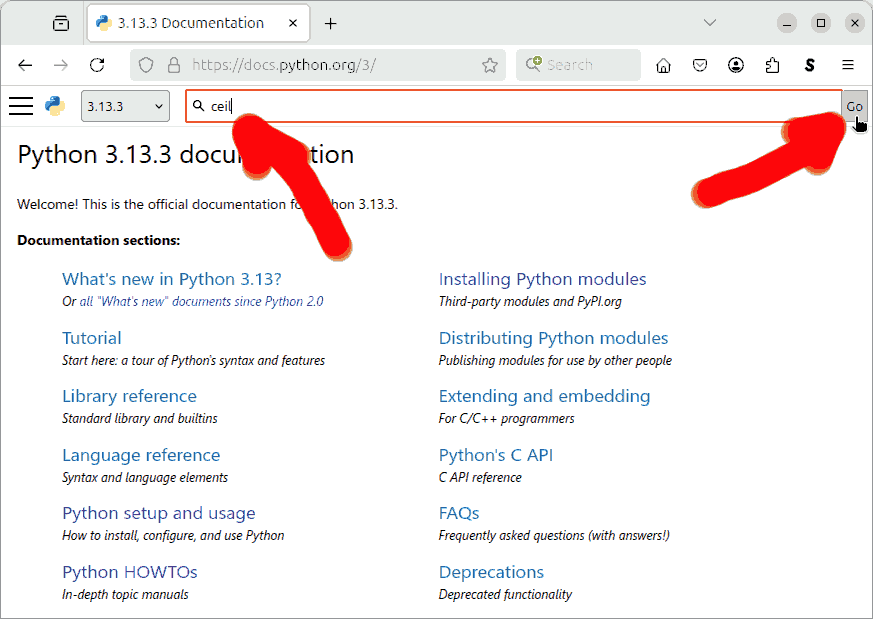
\includegraphics[width=0.47\linewidth]{\currentDir/pythondoc03searchCeil}}}%
%
\floatSep%
%
\subfloat[][%
Especially if you visit the website for the first time in your current web browser session, it may take some time until results show up. %
We wait patiently.%
\label{fig:pythondoc04wait}%
]{\tightbox{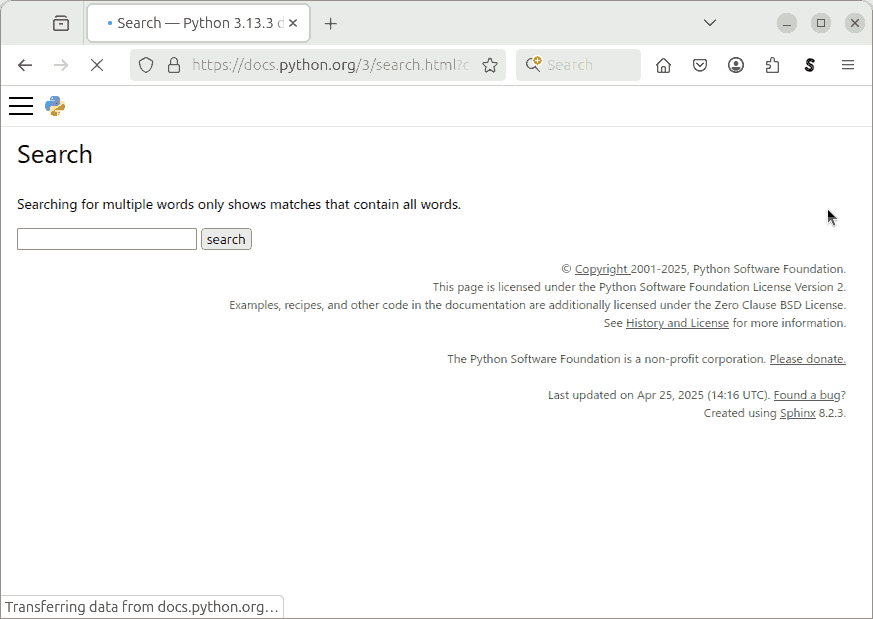
\includegraphics[width=0.47\linewidth]{\currentDir/pythondoc04wait}}}%
%
\floatRowSep%
%
\subfloat[][%
A list of documentation articles about the \pythonilIdx{ceil} function appears. %
We click on the link to~\pythonil{math.ceil}.%
\label{fig:pythondoc05results}%
]{\tightbox{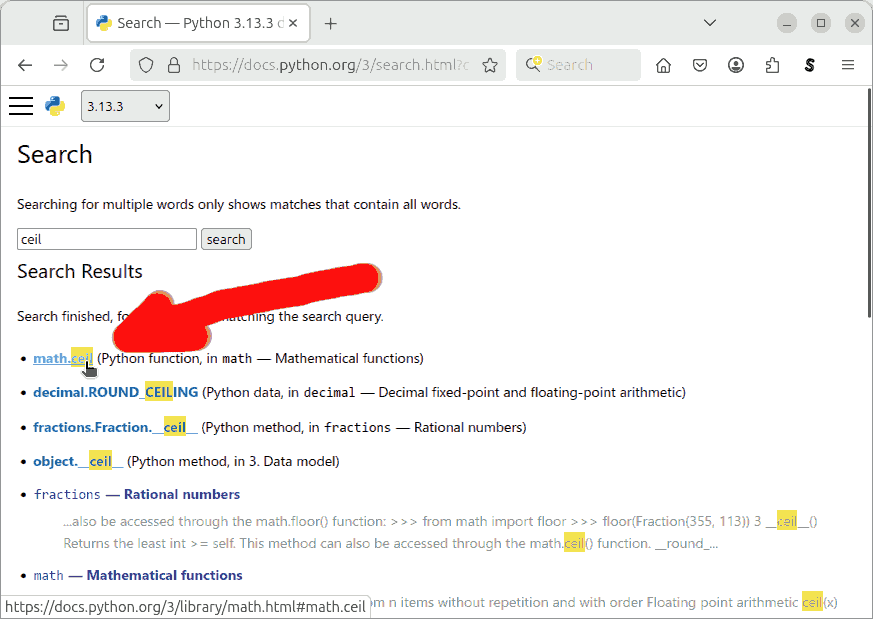
\includegraphics[width=0.47\linewidth]{\currentDir/pythondoc05results}}}%
%
\floatSep%
%
\subfloat[][%
It takes us to the \pythonilIdx{ceil}~entry of the \citetitle{PSF:P3D:TPSL:MMF} page~\cite{PSF:P3D:TPSL:MMF} at \citeurl{PSF:P3D:TPSL:MMF}. %
Indeed, we find a brief explanation about the \pythonilIdx{ceil} function.~%
(Also, we find a link to further reading about the \dunder{ceil} method, which we will discuss much later in~\cref{fig:pythonDunder:2}.)
\label{fig:pythondoc06mathceil}%
]{\tightbox{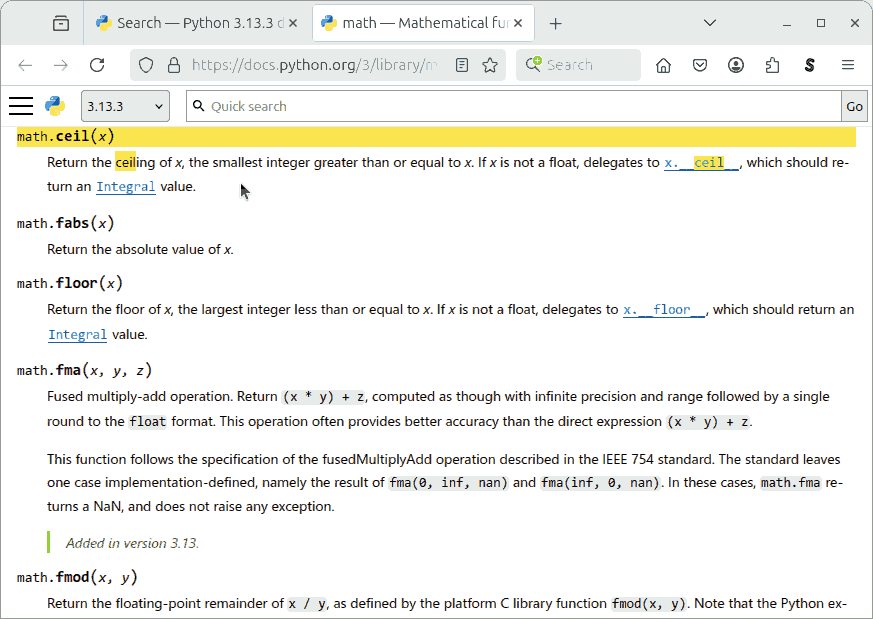
\includegraphics[width=0.47\linewidth]{\currentDir/pythondoc06mathceil}}}%
%
%
\caption{Searching the \citetitle{PSF:P3D}~\cite{PSF:P3D} for information about the function~\pythonilIdx{ceil}.}%
\label{fig:pythondoc:A}%
\end{noglslink}%
\end{figure}%
%
The answer to the first question is rather simple:
There is a complete online help catalog available for \python:~the \citetitle{PSF:P3D}~\cite{PSF:P3D} at~\citeurl{PSF:P3D}.
This should be your primary destination if you want to learn anything about \python.
Also, it is available in Chinese.

As example, let us imagine that you want to learn more about the function~\pythonilIdx{ceil}.
In \cref{fig:pythondoc01website}, we open a browser and visit the \citetitle{PSF:P3D}~\cite{PSF:P3D} at~\url{https://docs.python.org/3}.
On this page, you will either directly see a drop-down box where you can choose your favorite language or you can find it by clicking the \menu{\threeBarButton} at on the top-left corner of the website.
In the menu that opens in \cref{fig:pythondoc02language}, you can change the language and, e.g., select simplified Chinese~(简体中文)~\cite{SCR1956ROTSCOPTSCCS1} if that is your preferred language.
I will not do so and instead continue here in English.

Regardless of which language you chose, we still want to find information about the \pythonilIdx{ceil}~function.
Therefore, we locate the search bar \emph{in the website}~(not the one where you type in the \pglspl{URL} in the web browser).
Into this search bar, we type \pythonilIdx{ceil} and click on~\menu{Go} in \cref{fig:pythondoc03searchCeil}.

Depending on your internet connection and your location on the globe, it may take a bit of time until results are displaced.
Especially when visiting the page for the first time during a browsing session.
We wait patiently in \cref{fig:pythondoc04wait}.
And indeed, a list of documentation articles about the \pythonilIdx{ceil} function appears after a brief wait in \cref{fig:pythondoc05results}.
We decide that the link to \pythonil{math.ceil} looks most promising and click on it.

It takes us to the \pythonilIdx{ceil}~entry of the \citetitle{PSF:P3D:TPSL:MMF} page~\cite{PSF:P3D:TPSL:MMF} at \citeurl{PSF:P3D:TPSL:MMF}.
There, we find a brief explanation about the \pythonilIdx{ceil} function, as shown in \cref{fig:pythondoc06mathceil}.
The explanation also provides further reading, e.g., a link to the \dunder{ceil} method.
This is not important here, we will discuss it much later in~\cref{fig:pythonDunder:2}, but if we were interested, we could continue exploring and find more information about~\pythonilIdx{ceil}.
Also, we see that the information about the \pythonilIdx{ceil}~function is part of a longer list of mathematical functions.
Being curious, we would scroll a bit through this list.
Maybe we could learn about one or two other functions that we did not know about yet.%
%
\usefulTool{pythonDoc}{%
The first place to look for information about \python\ is the official \citetitle{PSF:P3D} at \citeurl{PSF:P3D}. %
This is the \emph{authoritative} source about \python: %
Everything what is written there is \emph{true} and \emph{exact} regarding~\python. %
All other sources may contain errors, be imprecise, ambiguous, or outdated. %
Therefore, always first consult the official \python\ documentation when being in doubt or looking for information.%
}%
%
Of course, in many cases, we do not know the name of the function we are looking for.
Assume that you did not know that the function~\pythonilIdx{ceil} exists.
You were looking for a way to round floating point numbers \inQuotes{upwards.}

You want to do something that you know should somehow be possible.
You think that \python\ should probably offer some out-of-the-box function for doing that.
If not, there should at least be some \inQuotes{standard \python way} to do that.
Anyway, the point is:
You do not have a function name to look for.

Let's again start at the search mask of the \citetitle{PSF:P3D} at~\citeurl{PSF:P3D}.
In \cref{fig:rounding01searchInDocumentation}, we try to describe what we want to do as clearly as possible.
\inQuotes{Rounding up} is maybe not very precise.
Let's enter \inQuotes{round towards positive infinity} into the search mask.

Sadly, the results shown in \cref{fig:rounding02foundNothingUseful} are not too useful.
This can happen.
The first result is unrelated to floating point numbers.
It offers us some discussion about objects implementing fractional arithmetics in a different way.
While we could find some hints in this text, it is not useful.

The second search result takes us to the a complete list of all functions in the module~\pythonilIdx{math}~\cite{PSF:P3D:TPSL:MMF}, but \emph{not} to the \pythonilIdx{ceil} function.
This means that we would need to go through the whole list of functions, read all of their descriptions, until we arrive at one that matches our goals.
This is a feasible method.
The list is not too long.
We could indeed spot the right answer here.
And we would probably learn more about \python\ on the way.
So directly working our way through the documentation here is a good idea.%
%
\FloatBarrier%
\endhsection%
%
\hsection{Searching for Second-Hand Information in the Web}%
\begin{figure}%
\centering%
\begin{noglslink}%
%
\subfloat[][%
We try searching for information about \inQuotes{round towards positive infinity} in the~\citetitle{PSF:P3D}~\cite{PSF:P3D} at~\citeurl{PSF:P3D}.%
\label{fig:rounding01searchInDocumentation}%
]{\tightbox{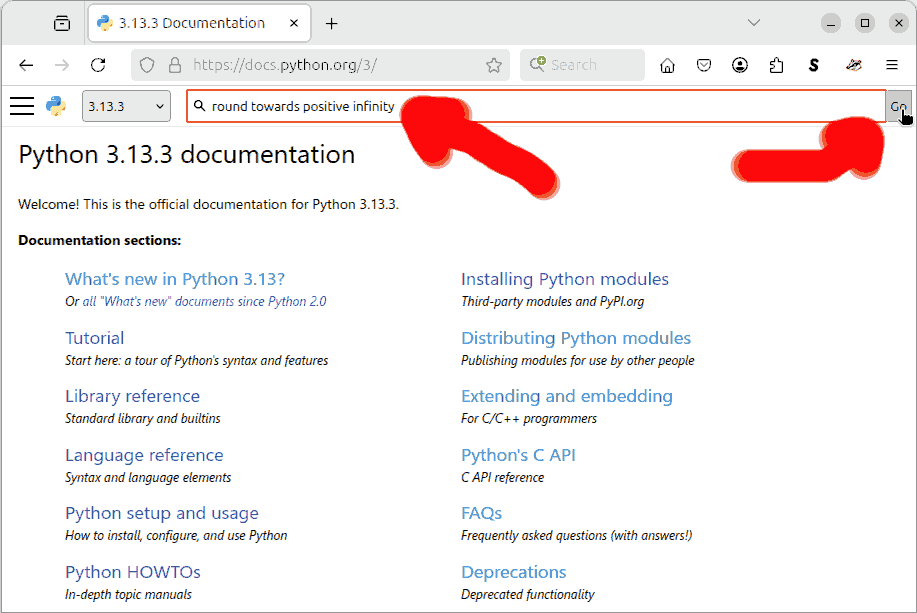
\includegraphics[width=0.47\linewidth]{\currentDir/rounding01searchInDocumentation}}}%
%
\floatSep%
%
\subfloat[][%
The results are not too useful. %
The first result is unrelated to floating point numbers. %
The second one is a complete list of all functions in the module~\pythonilIdx{math}. %
However, without knowing that the right function is called~\pythonilIdx{ceil}, finding it in this list could be hard.%
\label{fig:rounding02foundNothingUseful}%
]{\tightbox{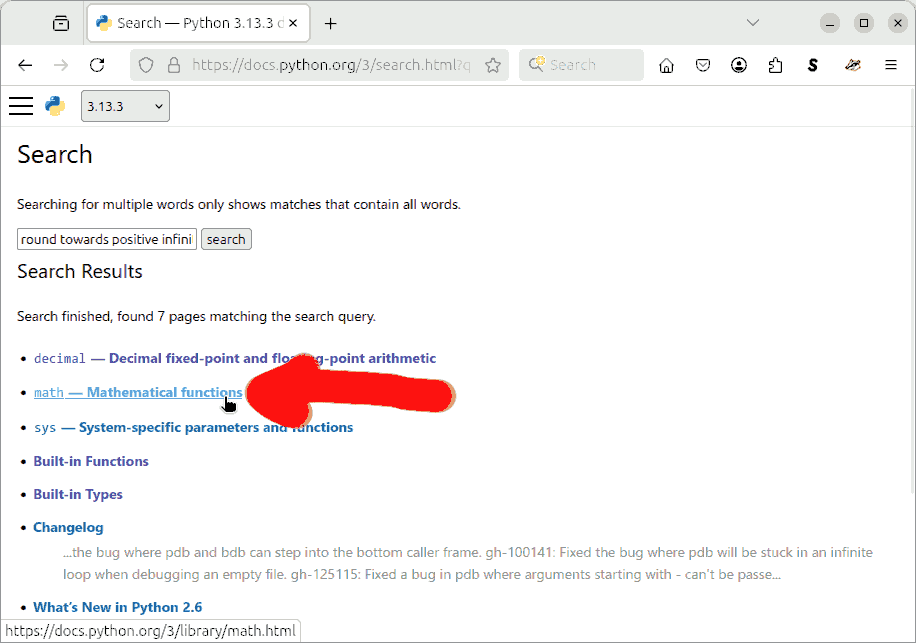
\includegraphics[width=0.47\linewidth]{\currentDir/rounding02foundNothingUseful}}}%
%
\floatRowSep%
%
\subfloat[][%
We enter \inQuotes{round towards positive infinity} into an internet search engine, here Microsoft Bing at~\url{https://bing.com}, but any search engine should do just as well. %
The result looks promising.%
\label{fig:rounding03searchEngine}%
]{\tightbox{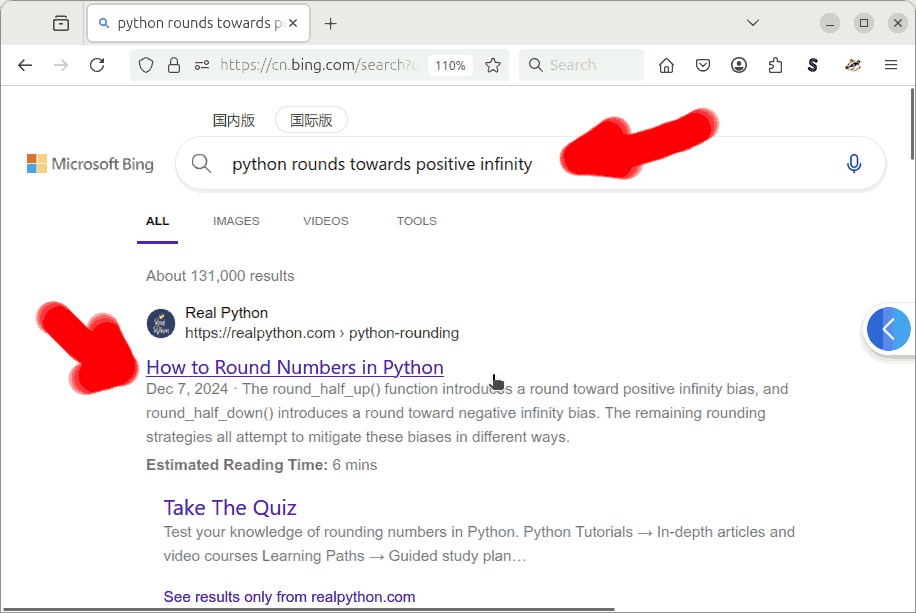
\includegraphics[width=0.47\linewidth]{\currentDir/rounding03searchEngine}}}%
%
\floatSep%
%
\subfloat[][%
Clicking on the first result, we visit the page~\citetitle{D2021RPT:A2024HTRNIP}~\cite{D2021RPT:A2024HTRNIP} at \citeurl{D2021RPT:A2024HTRNIP}.%
\label{fig:rounding04realPython}%
]{\tightbox{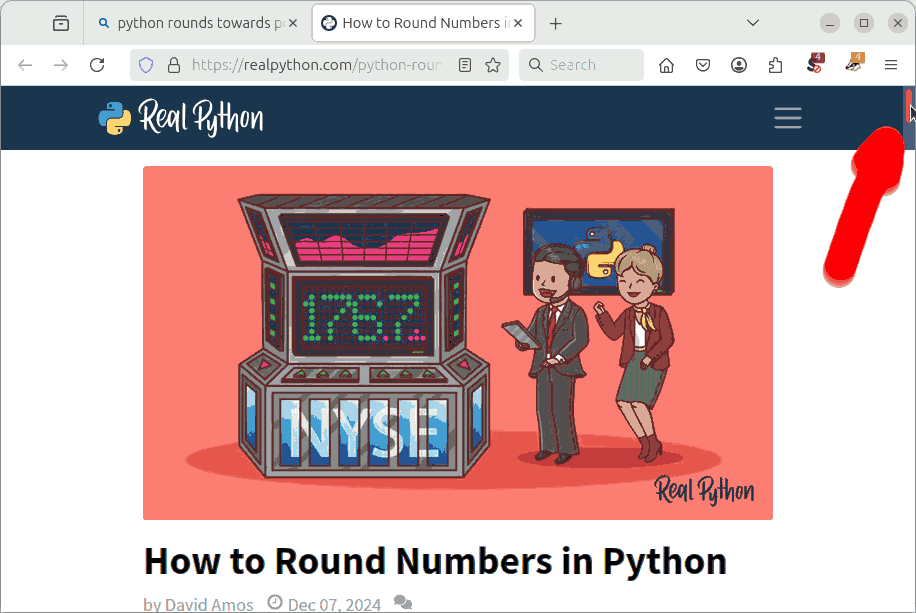
\includegraphics[width=0.47\linewidth]{\currentDir/rounding04realPython}}}%
%
\floatRowSep%
%
\subfloat[][%
After scrolling down a bit, we indeed find the information we want: %
For rounding up, the function~\pythonilIdx{ceil} is suitable. %
It is even presented as hyperlink.%
\label{fig:rounding05realPythonScrolledToCeil}%
]{\tightbox{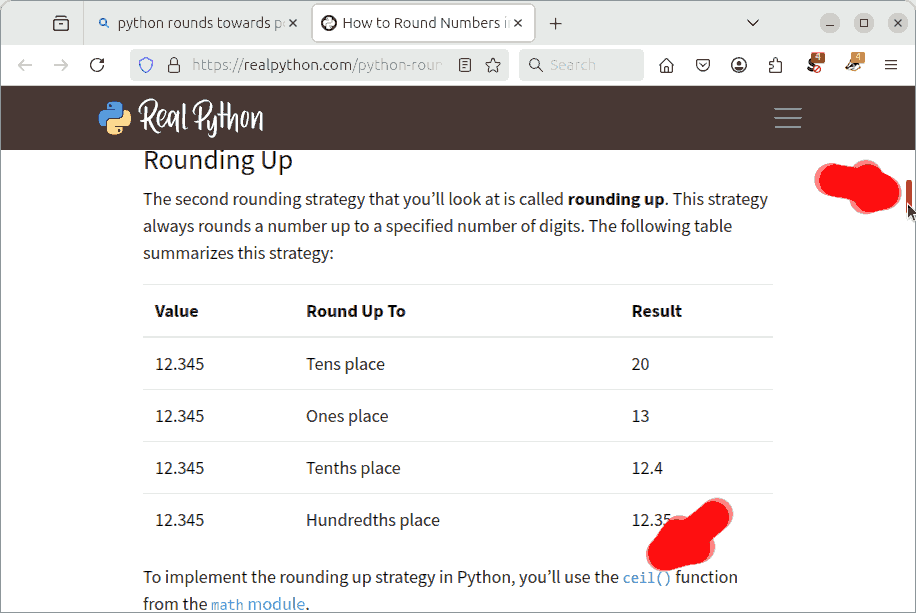
\includegraphics[width=0.47\linewidth]{\currentDir/rounding05realPythonScrolledToCeil}}}%
%
\floatSep%
%
\subfloat[][%
If we click on the hyperlink, it takes us to the \pythonilIdx{ceil}~entry in the \citetitle{PSF:P3D:TPSL:MMF} page~\cite{PSF:P3D:TPSL:MMF} at \citeurl{PSF:P3D:TPSL:MMF}.%
\label{fig:rounding06foundCeilInPythonDoc}%
]{\tightbox{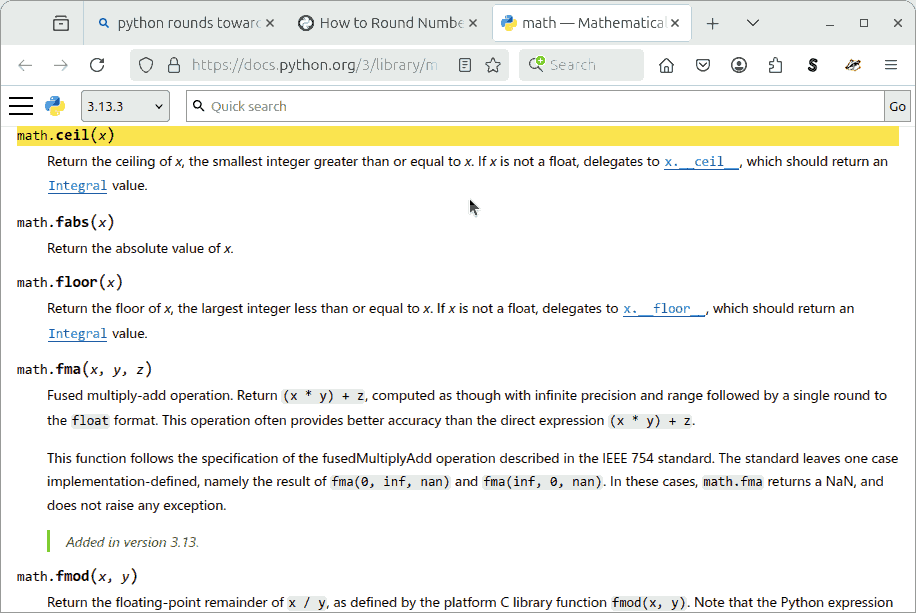
\includegraphics[width=0.47\linewidth]{\currentDir/rounding06foundCeilInPythonDoc}}}%
%
\caption{Searching for a \python\ function for \inQuotes{rounding up} if we do not know its name by using a search engine.}%
\label{fig:pythondoc:B}%
\end{noglslink}%
\end{figure}%
%
But let's say that we did not find anything useful and gave up using the \python\ documentation directly.
The second thing that we could try is to enter the description of what we want to do into a common search engine.
In \cref{fig:rounding03searchEngine}, we use Microsoft Bing at~\url{https://bing.com}, but any other search engine would probably be as same as good.
We enter \inQuotes{round towards positive infinity} into the search mask and hit~\menu{Search}.

The first result looks promising right way:~\citetitle{D2021RPT:A2024HTRNIP}.
While it does not say \inQuotes{round towards infinity,} if it summarizes all information about rounding numbers as the title indicates, then that topic is bound to come up somewhere.
So we click the link.

It takes us visit to the page~\citetitle{D2021RPT:A2024HTRNIP}~\cite{D2021RPT:A2024HTRNIP} at \citeurl{D2021RPT:A2024HTRNIP} in \cref{fig:rounding04realPython}.
A summary page on all about rounding of numbers.
Nice.

We begin to read the text.
Reading is an important skill, as reading texts and tutorials can significantly expand our knowledge.
After reading for a while, we indeed find the information we want:
For rounding up, the function~\pythonilIdx{ceil} is suitable.
It is even presented as a hyperlink in \cref{fig:rounding05realPythonScrolledToCeil}.
If we click on the hyperlink in \cref{fig:rounding06foundCeilInPythonDoc}, it takes us to the \pythonilIdx{ceil}~entry in the \citetitle{PSF:P3D:TPSL:MMF} page~\cite{PSF:P3D:TPSL:MMF} at \citeurl{PSF:P3D:TPSL:MMF}.
So we went round trip:
Even if we do not know how to do a given thing or what its name is, we can still find our way to the \python\ documentation.%
%
\usefulTool{searchEngines}{%
Search engines are useful tools to find information about certain functionality. %
Writing a precise description of the problem or functionality into the search bar of a search engine can lead to pages that describe answers or take us to the official \python\ documentation. %
However, search engines can also lead us to pages containing wrong, incomplete, ambiguous, outdated, or otherwise useless information. %
It is important to compare whatever information we found with the official \python\ documentation~\cite{PSF:P3D}~(see also~\cref{bp:searchAndLLM}).%
}%
%
\begin{figure}%
\centering%
\begin{noglslink}%
%
\subfloat[][%
We visit \citetitle{SE:SO}~\cite{SE:SO} at \citeurl{SE:SO}. %
(Sometimes we get asked to load some \pgls{javascript} from additional sources, which we click OK.)%
\label{fig:stackOverflow01websiteLoading}%
]{\tightbox{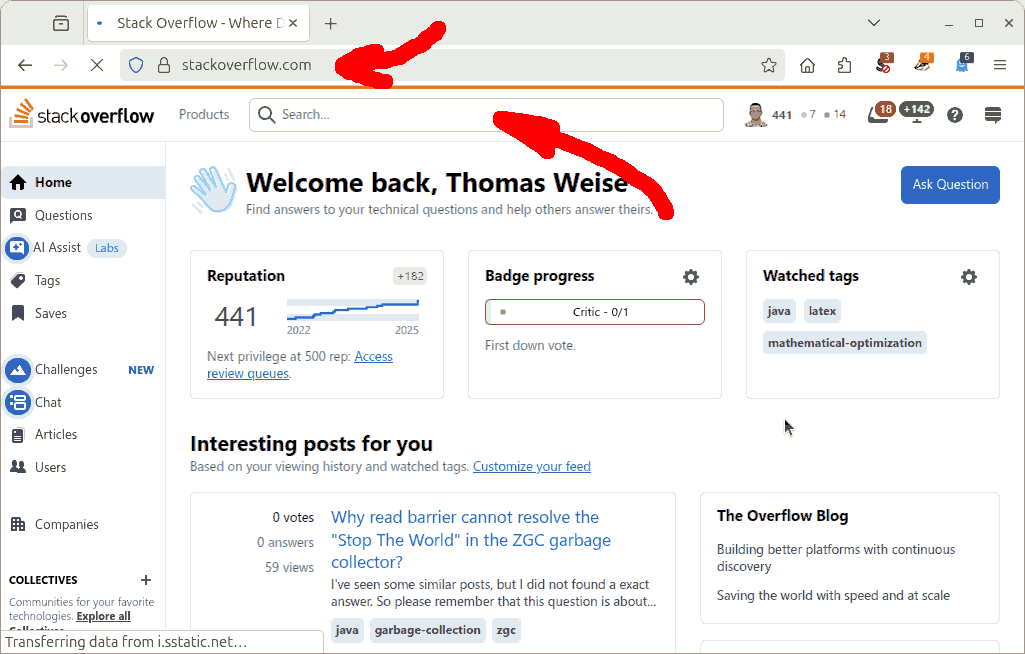
\includegraphics[width=0.47\linewidth]{\currentDir/stackOverflow01websiteLoading}}}%
%
\floatSep%
%
\subfloat[][%
The website has loaded, we can click into the search field to enter a query.%
\label{fig:stackOverflow02websiteLoadedEnterQuery}%
]{\tightbox{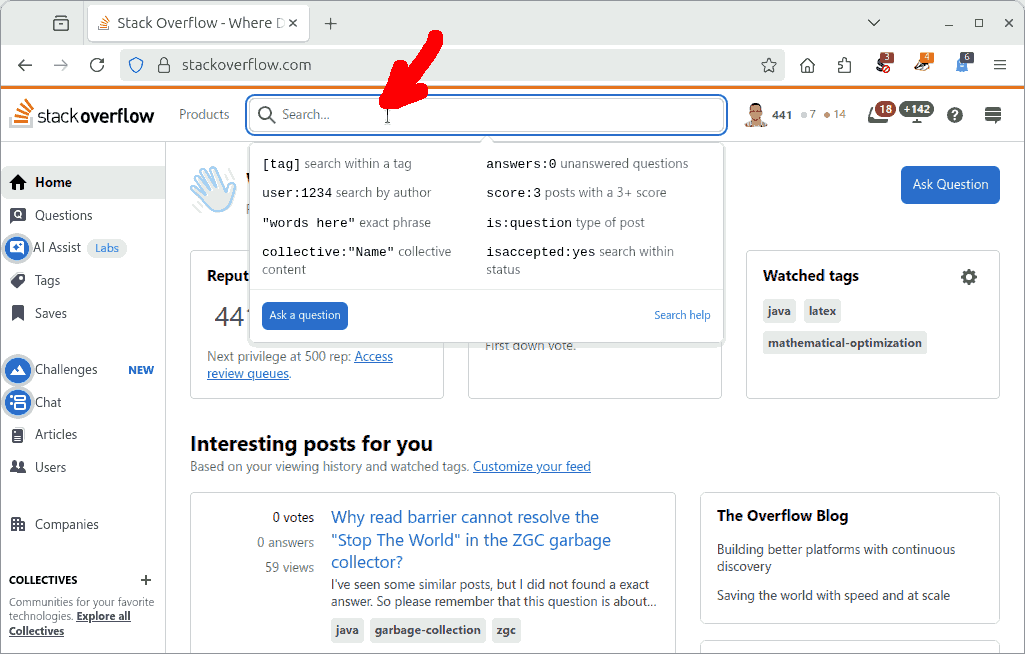
\includegraphics[width=0.47\linewidth]{\currentDir/stackOverflow02websiteLoadedEnterQuery}}}%
%
\floatRowSep%
%
\subfloat[][%
We enter our query \emph{\inQuotes{python rounding towards infinity}} and press~\keys{\enter}.%
\label{fig:stackOverflow03queryEntered}%
]{\tightbox{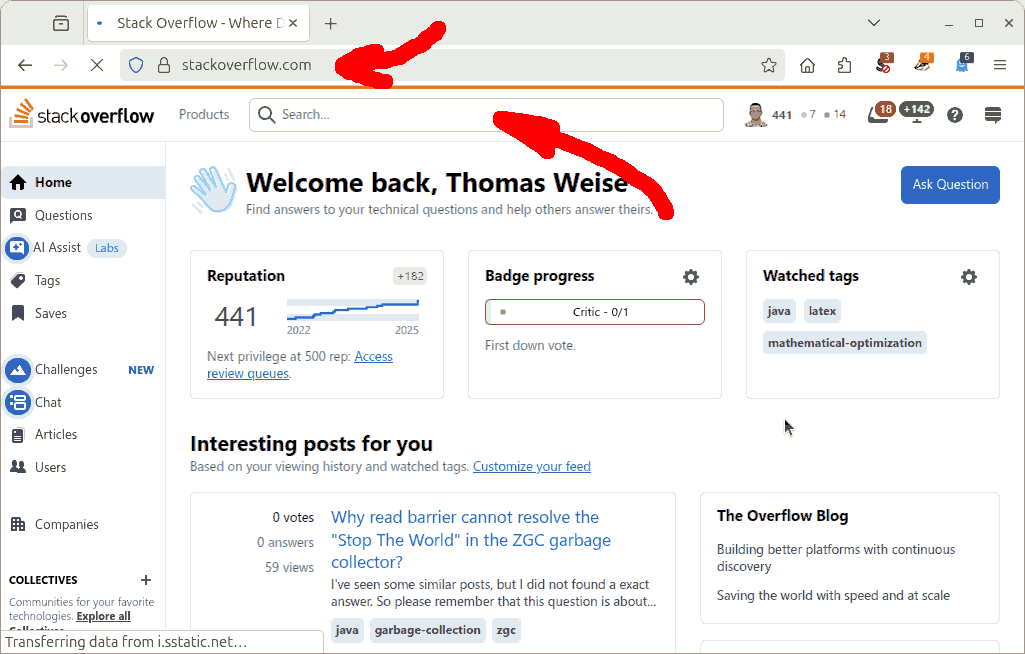
\includegraphics[width=0.47\linewidth]{\currentDir/stackOverflow01websiteLoading}}}%
%
\floatSep%
%
\subfloat[][%
The questions that are similar to our query are displayed. %
The first few look unrelated. %
We scroll down.%
\label{fig:stackOverflow04queryAnsweres}%
]{\tightbox{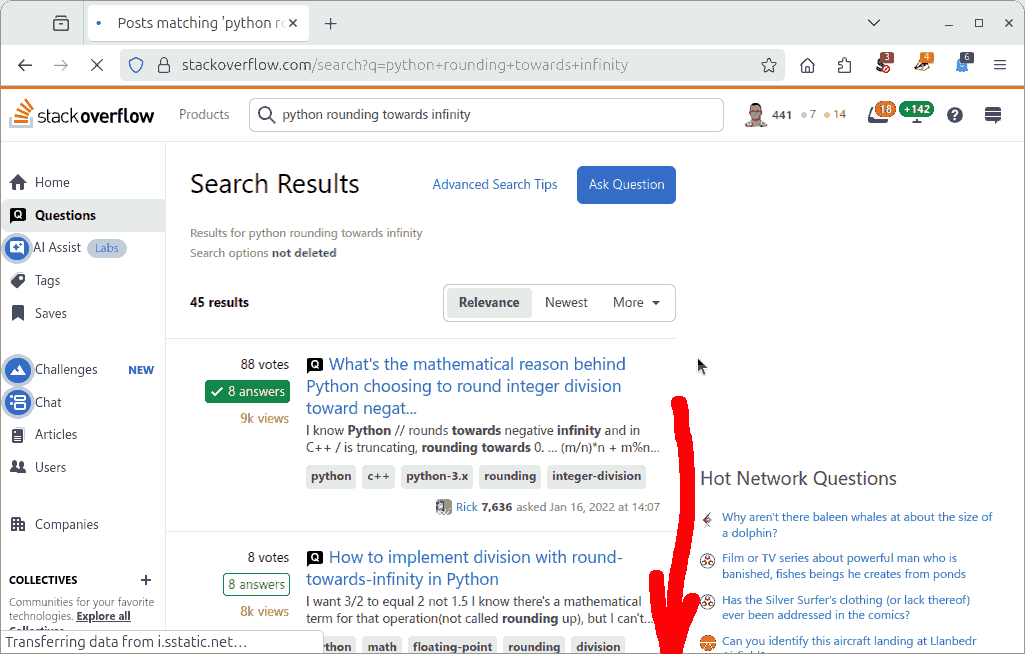
\includegraphics[width=0.47\linewidth]{\currentDir/stackOverflow04queryAnsweres}}}%
%
\floatRowSep%
%
\subfloat[][%
We find the vaguely related-sounding question \citetitle{SE:SO:HTIDWRTIIP}~\cite{SE:SO:HTIDWRTIIP} and click on it.%
\label{fig:stackOverflow05foundVaguelyRelatedQuestion}%
]{\tightbox{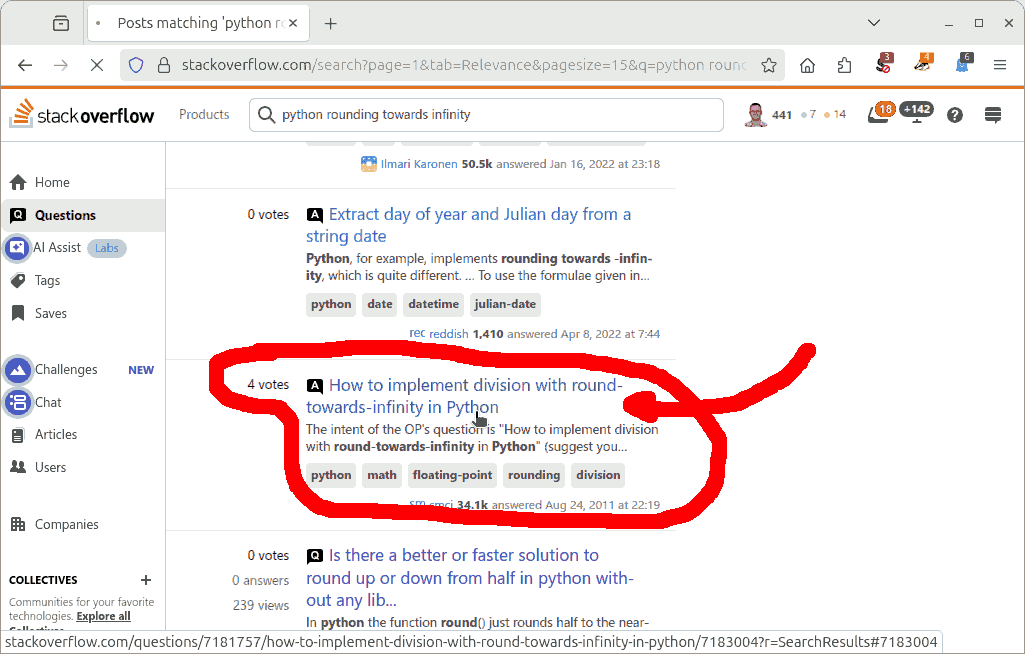
\includegraphics[width=0.47\linewidth]{\currentDir/stackOverflow05foundVaguelyRelatedQuestion}}}%
%
\floatSep%
%
\subfloat[][%
Indeed, the question fits {\dots} but its explanation of the division operator does not fit to our understanding of it. %
We realize that it is from \citeyear{SE:SO:HTIDWRTIIP} and about \python~2.%
\label{fig:stackOverflow06questionFits}%
]{\tightbox{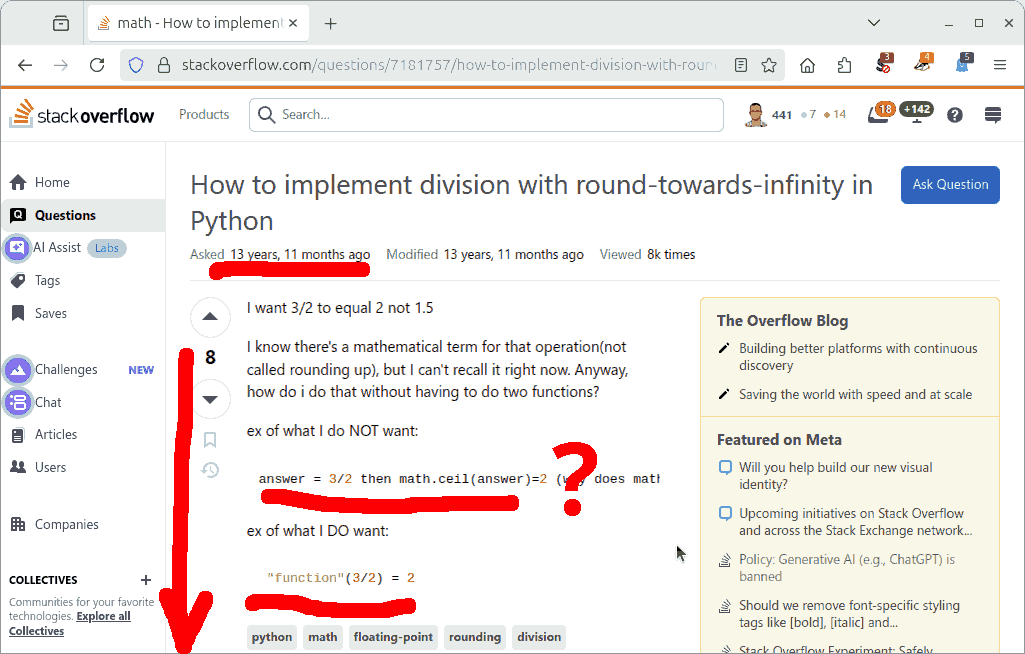
\includegraphics[width=0.47\linewidth]{\currentDir/stackOverflow06questionFits}}}%
%
\floatRowSep%
%
\subfloat[][%
Scrolling to the answers of the question, we find an explanation of this issue and a pointer to an authoritative source~\cite{PEP238} explaining it. %
We also find the \pythonilIdx{ceil}\pythonIdx{math!ceil} function. %
We can now look it up in the \python~3 documentation.%
\label{fig:stackOverflow07solutionFits}%
]{\parbox{0.99\linewidth}{\centering%
\tightbox{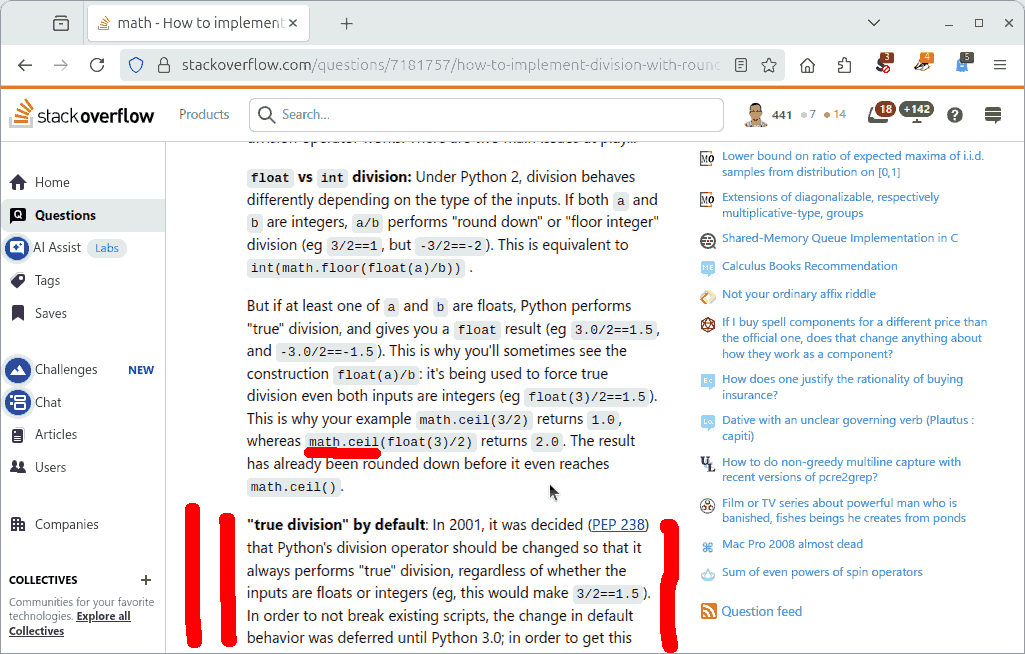
\includegraphics[width=0.47\linewidth]{\currentDir/stackOverflow07solutionFits}}}}%
%
\caption{Using \citetitle{SE:SO} to find information how to \inQuotes{round up} \pythonils{float} in \python.}%
\label{fig:searchingForInfosUsingSO}%
\end{noglslink}%
\end{figure}%
%
Another group of possible sources for information on how to solve a certain programming problem or what command can be used to achieve a certain effect are dedicated websites for programming.
The maybe most well-known is \citetitle{SE:SO}~\cite{SE:SO} at \citeurl{SE:SO}.
This is a website where programmers can ask and answer programming questions.
Let's see whether we can use it to find a way to round numbers toward infinity in \python.

One such attempt is illustrated in \cref{fig:searchingForInfosUsingSO}.
There, we visit the \citetitle{SE:SO} website and enter our query \emph{\inQuotes{python rounding towards infinity.}}
This will show us several pages of questions that programmers have asked in the past and which \citetitle{SE:SO} thinks are related to our issue.
We even find a question~\cite{SE:SO:HTIDWRTIIP} that sounds vaguely related to what we want to know.

Clicking on it, we notice that this question seems odd:
The author seems under the impression that \pythonilIdx{/} conducts an integer division, which we know is not true.
We know that \pythonilIdx{//} does integer divisions, but \pythonilIdx{/} produces~\pythonils{float}.
At first we are puzzled by this, but then notice that this question is from~\citeyear{SE:SO:HTIDWRTIIP}.
It targets \python~2, which, at that time, was the \inQuotes{only} \python.

Still, after scrolling down into the answers a bit, we find the whole issue explained.
The answers even point us to the authoritative source regarding the semantics of the division operators, namely PEP~238~\cite{PEP238}.
And we find the operator \pythonilIdx{ceil}!
Having found the name of the operator, we could now go back to the \python\ documentation as shown in \cref{sec:authorativeDoc}.
We can then look up the operator, get the information we need, and continue programming.

This example shows one more issue of non-authoritative sources:
They may be outdated.
Software is not static.
It changes and evolves.
This holds for the programs that we develop as well as for the programming languages themselves.

So any text that you find in the web -- including this book -- may be out of date when you read it.
The information it provides may be incomplete or not even correct anymore.
Therefore, circling back to the authoritative sources is always necessary after we found the hints we are looking for.%
%
\FloatBarrier%
\endhsection%
%
\hsection{Asking an AI for Answers}%
%
\begin{figure}%
\centering%
\begin{noglslink}%
%
\subfloat[][%
We open the BaiDu~(百度) search page at~\url{https://baidu.com} and click on \inQuotes{AI搜索已接入DeepSeek\nobreakdashes-V3最新版模型}.%
\label{fig:ai01baidu}%
]{\tightbox{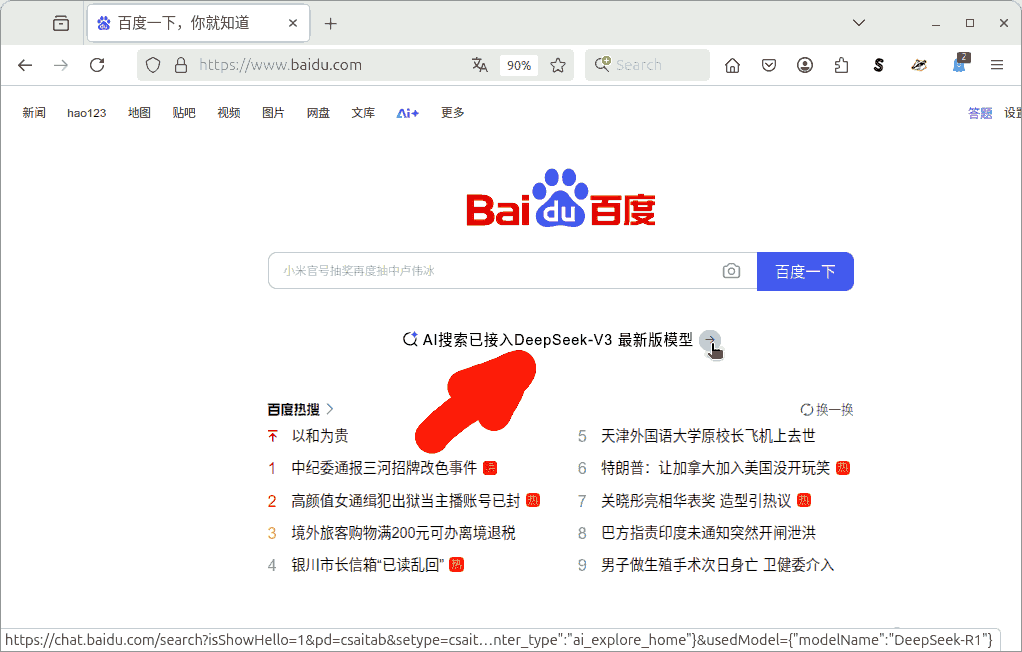
\includegraphics[width=0.47\linewidth]{\currentDir/ai01baidu}}}%
%
\floatSep%
%
\subfloat[][%
We arrive at the \inQuotes{Hi,AI搜索已支持R1满血版,快来试试吧!}~page where we can enter the prompt for the DeepSeek\nobreakdashes-R1 model~\cite{DAGYZSZXZMWBZYWWGSLGLXWWFLZDZRDCJLLDLHCLZBXWDXGQLGLWCYQLCNLCDHGGHYWZZWZXXZZTLWLTHZWCDGZPWCJCLZCYWYZPL2024DRIRCILVRL} in the input field at the bottom.%
\label{fig:ai02deepseek}%
]{\tightbox{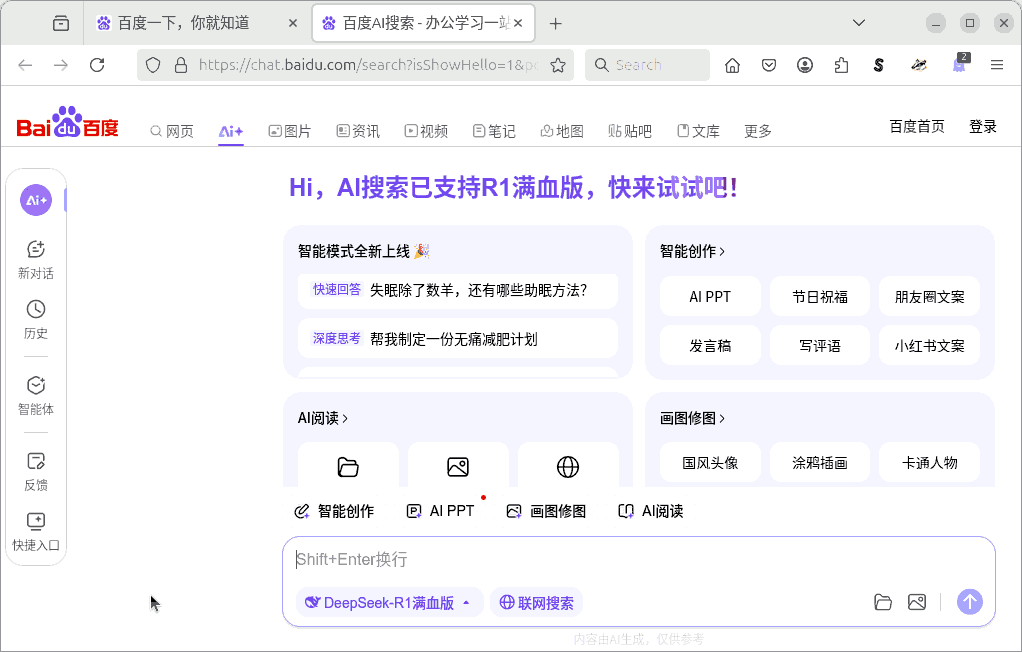
\includegraphics[width=0.47\linewidth]{\currentDir/ai02deepseek}}}%
%
\floatRowSep%
%
\subfloat[][%
We enter our query~\inQuotes{How can I round floating point numbers towards positive infinity in Python?} and execute it.%
\label{fig:ai03deepseekQuery}%
]{\tightbox{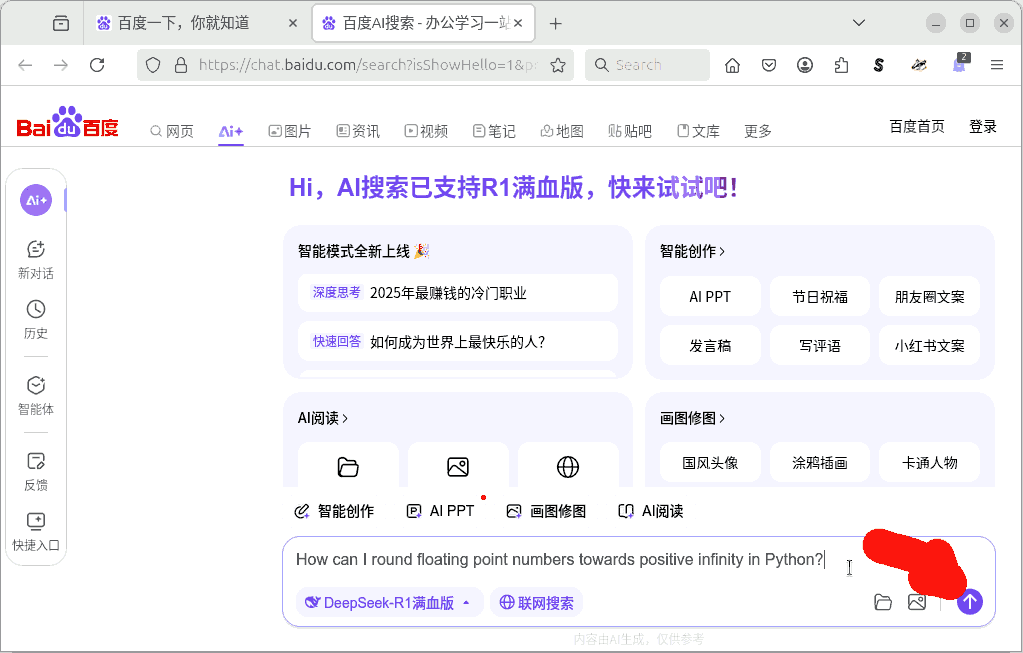
\includegraphics[width=0.47\linewidth]{\currentDir/ai03deepseekQuery}}}%
%
\floatSep%
%
\subfloat[][%
DeepSeek responds with a long answer of over 1700~words of text, as illustrated in \cref{fig:deepseek:output}.%
\label{fig:ai04deepseekAnswer1}%
]{\tightbox{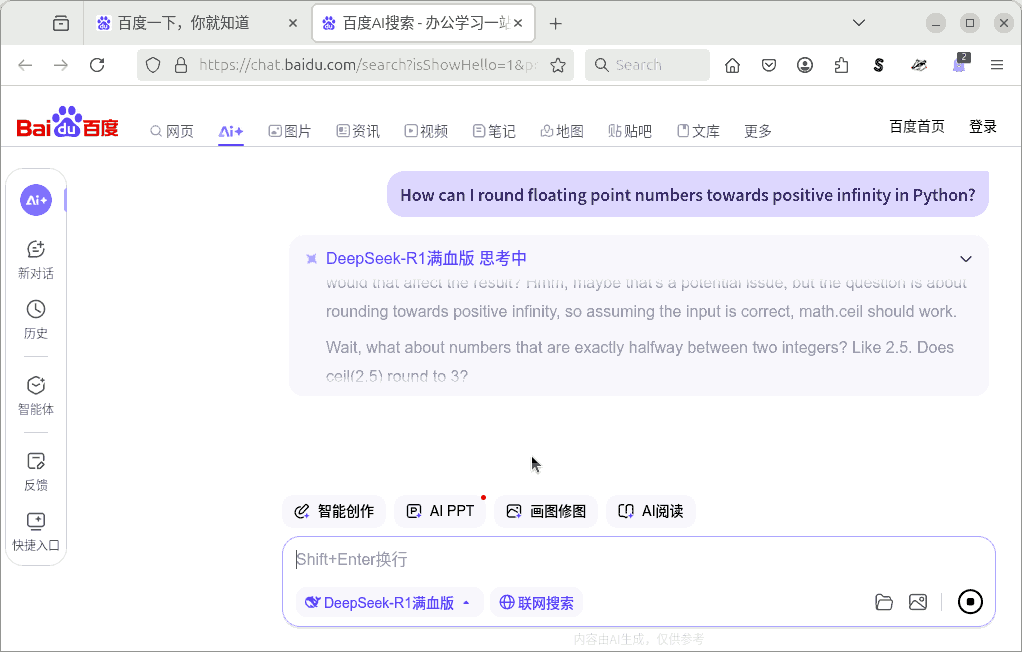
\includegraphics[width=0.47\linewidth]{\currentDir/ai04deepseekAnswer1}}}%
%
\floatRowSep%
%
\subfloat[][%
But it still and early on correctly points us to \pythonil{math.ceil} plus it shows this information prominently in the text.%
\label{fig:ai05deepseekAnswer2}%
]{\tightbox{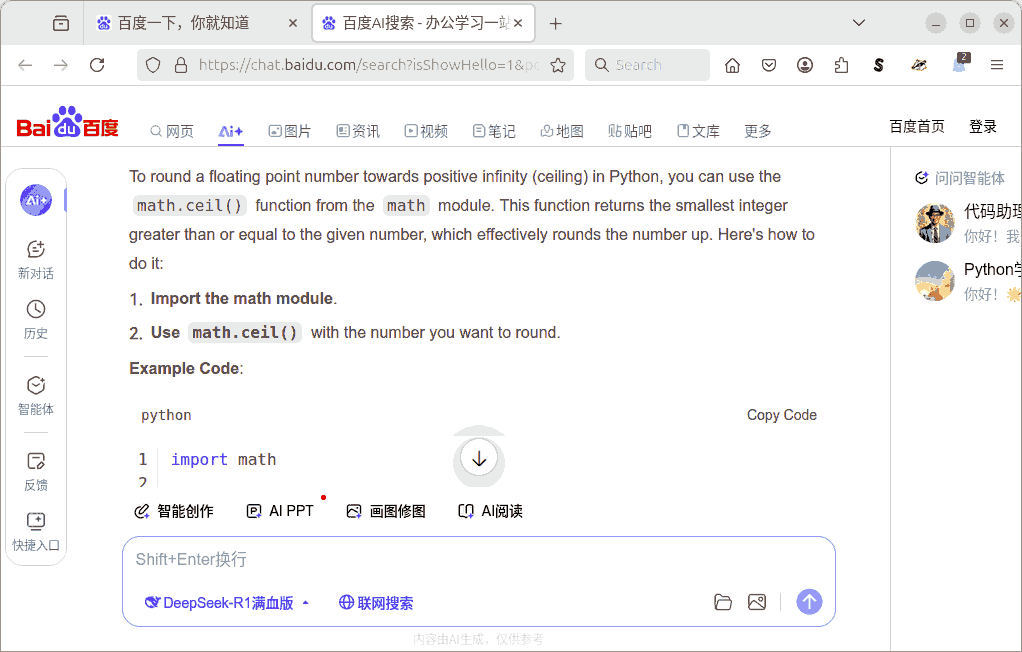
\includegraphics[width=0.47\linewidth]{\currentDir/ai05deepseekAnswer2}}}%
%
\floatSep%
%
\subfloat[][%
And it even provides a small snippet of code.%
\label{fig:ai06deepseekAnswer3}%
]{\tightbox{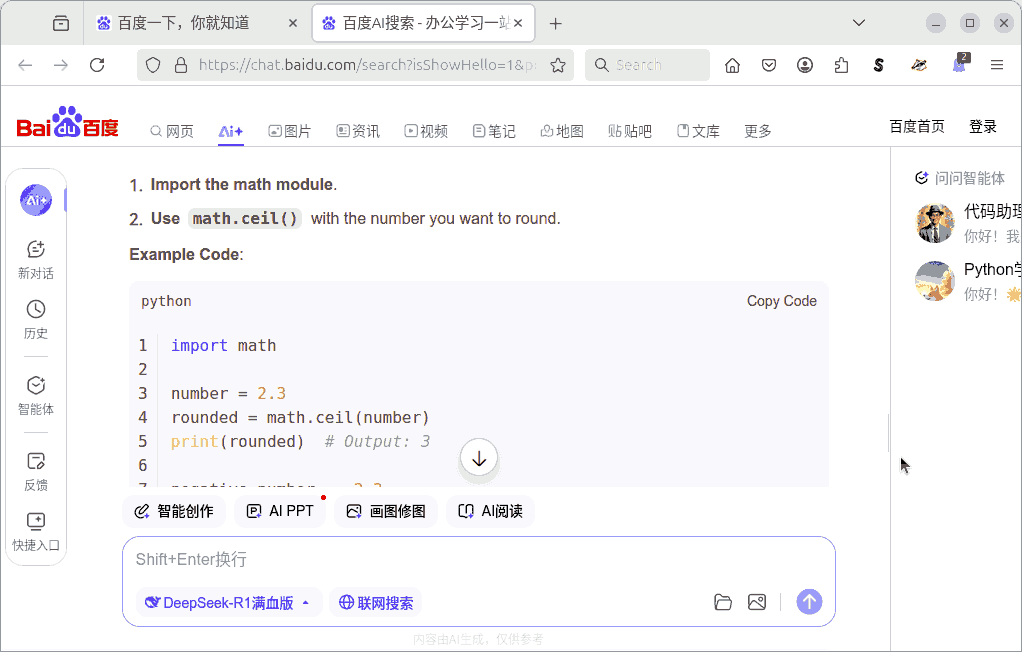
\includegraphics[width=0.47\linewidth]{\currentDir/ai06deepseekAnswer3}}}%
%
\caption{Searching for a \python\ function for \inQuotes{rounding up} if we do not know its name by using an~\pgls{AI}.}%
\label{fig:pythondoc:C}%
\end{noglslink}%
\end{figure}%
%
\begin{figure}%
\centering%
\begin{noglslink}%
\fcolorbox{yellow!20!black}{yellow!10!white}{%
\resizebox{0.97\linewidth}{!}{%
\begin{minipage}{1.12\linewidth}%
{\tiny{Okay, I need to figure out how to round floating point numbers towards positive infinity in Python.
Let's see, rounding towards positive infinity is also known as ceiling.
{\color{blue}{So, maybe there's a function called \texttt{ceil} in Python?}}\smallskip

Wait, I remember that Python has a \texttt{math} module.
Let me check.
{\color{blue}{Yes, the \texttt{math} module has a \texttt{ceil} function.}}
So, \texttt{math.ceil()} should do the trick.
But wait, how does it handle different numbers?
For example, if the number is already an integer, does it leave it as is?
And for negative numbers, does it round them up towards zero or away?\smallskip

Let me think.
The ceiling function in mathematics rounds a number up to the nearest integer.
So, for positive numbers, even if they are already integers, it stays the same.
For negative numbers, it would round towards zero.
For example, \texttt{ceil(-2.3)} would be \texttt{-2}, which is greater than \texttt{-2.3}.
So that's correct for positive infinity direction.\smallskip

{\color{red}{But how about when dealing with floating points that are very close to an integer due to precision issues?
Like \texttt{2.0000000001}, would \texttt{ceil} round it to \texttt{3}?
Probably not, because the function should handle that as per the actual value.}}
Wait, but floating points can have precision problems.
For instance, \texttt{1.1} might not be represented exactly.
So \texttt{ceil(1.1)} should give \texttt{2}, but if due to some calculation the number is actually stored as slightly less than \texttt{1.1}, would that affect the result?
Hmm, maybe that's a potential issue, but the question is about rounding towards positive infinity, so assuming the input is correct, \texttt{math.ceil} should work.\smallskip

Wait, what about numbers that are exactly halfway between two integers?
Like \texttt{2.5}.
Does \texttt{ceil(2.5)} round to \texttt{3}? Yes, because ceil rounds up regardless of the fractional part.
So, even \texttt{2.1} would go to \texttt{3}, right?
No, wait: \texttt{ceil(2.1)} is \texttt{3}?
No, wait no.
Wait, \texttt{ceil(2.1)} is \texttt{3}?
Wait no!
Wait, no.
Wait, no, that's not right.
Wait, the ceiling function rounds up to the smallest integer greater than or equal to the number.
So, \texttt{2.1}'s ceiling is \texttt{3}?
No, wait, \texttt{2.1} is between \texttt{2} and \texttt{3}.
The smallest integer greater than or equal to \texttt{2.1} is \texttt{3}?
Wait, no.
Wait \texttt{2.1} is greater than \texttt{2}, so the smallest integer greater or equal is \texttt{3}?
Wait, no, wait, \texttt{2.1}'s ceiling is \texttt{3}?
No, no.
Wait, \texttt{2.1} is between \texttt{2} and \texttt{3}.
So the ceiling is \texttt{3}.
Wait, but \texttt{2.0}'s ceiling is \texttt{2.0}.
So yes, \texttt{ceil(2.1)} would be \texttt{3}?
Wait, wait, I'm getting confused.
Let me think again.\smallskip

Wait, the ceiling of \texttt{2.1} is \texttt{3}?
No, that's not right.
Wait, the ceiling function rounds up to the next integer.
So \texttt{2.1} would have a ceiling of \texttt{3}?
No, wait no.
Wait, no, the ceiling of \texttt{2.1} is \texttt{3}?
No, that's not correct.
Wait, \texttt{2.1} is \texttt{2.1}, so the smallest integer greater than or equal to \texttt{2.1} is \texttt{3}?
No! Wait, \texttt{2} is less than \texttt{2.1}, but \texttt{3} is greater than \texttt{2.1}.
Wait, no, \texttt{2.1} is between \texttt{2} and \texttt{3}.
The ceiling is the smallest integer that is greater than or equal.
So \texttt{3} is greater than \texttt{2.1}, but \texttt{2} is less than \texttt{2.1}.
So the ceiling would be \texttt{3}?
No, that's not right.
Wait, no, \texttt{2.1} is greater than \texttt{2}, so the ceiling is the smallest integer that is not less than the number.
So the ceiling is \texttt{3}?
Wait, no.
Wait, \texttt{2.1} is \texttt{2.1}, so the next integer up is \texttt{3}.
So yes, \texttt{ceil(2.1)} is \texttt{3}?
Wait, no.
Wait, I think I made a mistake here.
Because the ceiling of \texttt{2.1} is \texttt{3}?
No, the ceiling of \texttt{2.1} is actually \texttt{3}.
Wait, no, that's not correct.
Wait, the ceiling of \texttt{2.0} is \texttt{2.0}.
The ceiling of \texttt{2.0} is \texttt{2.0}.
For \texttt{2.1}, the next integer higher is \texttt{3.0}.
So \texttt{ceil(2.1)} is \texttt{3.0}.
Wait, but that's not right.
Wait, \texttt{2.1} is less than \texttt{3.0}, but the ceiling is the smallest integer greater than or equal.
So for example, \texttt{ceil(2.0)} is \texttt{2.0}, \texttt{ceil(2.1)} is \texttt{3.0}?
That can't be right.
Wait, maybe I'm mixing up ceiling and floor functions.
Wait, the floor function rounds down.
So \texttt{floor(2.1)} is \texttt{2}.
The ceiling function rounds up.
So \texttt{ceil(2.1)} is \texttt{3.0}?
That would be the case.
But that's a big jump, but yes.
For example, in Python:%
%
\begin{center}%
\parbox{0.7\linewidth}{%
\texttt{import math}\\%
\texttt{math.ceil(2.1)}\\%
\texttt{3}%
}\end{center}%
%
Is that true?
Let me check.
Wait, no, that's not correct.
Wait, I'm confusing something here.
Let me check an example.
Let me try to recall: \texttt{ceil(1.2)} is \texttt{2}?
No.
Wait, no.
Wait, \texttt{ceil(1.2)} is \texttt{2}.
Yes, because \texttt{2} is the smallest integer greater than or equal to \texttt{1.2}.
Wait, no.
Wait, \texttt{1.2} is between \texttt{1} and \texttt{2}.
So the smallest integer greater than or equal to \texttt{1.2} is \texttt{2}?
No, that's not correct.
Wait, \texttt{1.2} is greater than \texttt{1}, but \texttt{2} is larger than \texttt{1.2}, but the ``smallest integer greater than or equal to'' \texttt{1.2} is \texttt{2}?
No.
Wait, no.
Wait, the integers around \texttt{1.2} are \texttt{1} and \texttt{2}.
\texttt{1.2} is greater than \texttt{1}, so the smallest integer that is greater than or equal is \texttt{2}?
No.
Wait, no.
Wait, \texttt{1.2} is \texttt{1.2}, so the next integer higher is \texttt{2}.
So the ceiling is \texttt{2}.
Yes.
So \texttt{ceil(1.2)} is \texttt{2}.
So in that case, yes, that's correct.\smallskip

Wait, but then for numbers like \texttt{2.5}, \texttt{ceil(2.5)} is \texttt{3}.
So regardless of the decimal part, it rounds up.
So that's correct.\smallskip

But in Python, how does this work?
Let me think of code examples.
If I do:%
%
{\color{blue}{%
\begin{center}%
\parbox{0.7\linewidth}{%
\texttt{import math}\\%
\texttt{print(math.ceil(2.1)) \# should output 3?}%
}\end{center}}}%
%
Wait, but when I run this code, what's the actual output?
Wait, maybe I'm making a mistake here.
Let me check.\smallskip

Wait, actually, if I run \texttt{math.ceil(2.1)}, the result is \texttt{3}.
Let me confirm.\smallskip

Wait, no, wait, no.
Wait, in Python, \texttt{math.ceil(2.1)} returns \texttt{3.0}?
Let me think again.
Wait, no, \texttt{2.1}'s ceiling is \texttt{3.0}?
That can't be right.
Wait, maybe I'm thinking of the integer division or something else.
Wait, no. Wait, the ceiling function works as in mathematics.
So for any non-integer, the ceiling is the next integer higher.\smallskip

Wait, but \texttt{2.0}'s ceiling is \texttt{2.0}, \texttt{2.1}'s ceiling is \texttt{3.0}.
Wait, that's how the function works.
So, yes, \texttt{math.ceil(2.1)} would return \texttt{3.0}.\smallskip

But wait, in reality, when I test this in Python, maybe it's different.
Let me think.
Wait, perhaps I'm making a mistake here.
Wait, let's see:\smallskip

For example, \texttt{math.ceil(2.1)} returns \texttt{3}, but \texttt{math.ceil(2.0)} returns \texttt{2.0}.
So, yes.\smallskip

So, for any positive number with a fractional part, ceil will round it up to the next integer.
For negative numbers, \texttt{ceil} will round towards zero.
For example, \texttt{ceil(-1.2)} is \texttt{-1}, because \texttt{-1} is greater than \texttt{-1.2}, and is the smallest integer that satisfies that.\smallskip

So, \texttt{math.ceil} is the correct function to use here.
Therefore, the answer is to use \texttt{math.ceil} from the \texttt{math} module.\smallskip

But wait, the user asked how to round towards positive infinity.
So, for positive numbers, that's rounding up (\texttt{ceil}), but for negative numbers, rounding towards positive infinity would also require moving towards zero, which \texttt{ceil} does.
So, yes, \texttt{math.ceil()} is correct.\smallskip

But let me check another case.
For example, if the number is already an integer, like \texttt{5.0}, then \texttt{ceil(5.0)} is \texttt{5.0,} which is correct.
If it's a negative number with fractional part, like \texttt{-3.2}, \texttt{ceil(-3.2)} is \texttt{-3.0}, which is towards positive infinity (since \texttt{-3} is greater than \texttt{-3.2}).
So that's correct.\smallskip

So, the conclusion is:
to round a floating point number towards positive infinity in Python, use the \texttt{math.ceil()} function from the \texttt{math} module.
You need to import \texttt{math} and then call \texttt{math.ceil(number)}.
The function returns a \texttt{float} if the input is a \texttt{float}, but if you want an integer, you can cast it to an \texttt{int}.\smallskip

Wait, but \texttt{math.ceil(2.1)} returns \texttt{3.0}, which is a \texttt{float}.
So if you need an integer, you have to convert it.
For example, \texttt{int(math.ceil(2.1))} gives \texttt{3}.
But the question is about rounding the floating point number towards positive infinity.
So depending on whether the user wants the result as a \texttt{float} or integer, but the default behavior of \texttt{math.ceil} returns a \texttt{float} if the input is a \texttt{float}.
For example, \texttt{math.ceil(2)} (if \texttt{2} is an integer) would return \texttt{2}, but if you pass \texttt{2.0}, it returns \texttt{2.0}.\smallskip

So the user needs to be aware of that.
But the main answer is to use \texttt{math.ceil}.\smallskip

Wait, but what about numbers that are already integers?
For example, \texttt{3.0}, \texttt{math.ceil(3.0)} returns \texttt{3.0}.
So if the user wants to ensure it's an integer, they can cast it.
But maybe the user just wants to round towards positive infinity, regardless of data type.\smallskip

So, the answer is to import math and use \texttt{math.ceil()}.\smallskip

Another thing to consider:
what if the number is very large and cannot be represented as an integer?
For example, \texttt{1e300} is a float, and \texttt{math.ceil(1e300)} would return the same \texttt{float}, which is the integer value.
But since Python can handle arbitrarily large integers, converting it to an integer would be possible.\smallskip

So, in summary, the way to round a floating point number towards positive infinity in Python is to use the \texttt{math.ceil} function.
Make sure to import the math module first.\smallskip

To round a floating point number towards positive infinity (ceiling) in Python, you can use the \texttt{math.ceil()} function from the math module.
This function returns the smallest integer greater than or equal to the given number, which effectively rounds the number up.
Here's how to do it:%
%
\begin{enumerate}%
\item Import the \texttt{math} module.%
\item Use \texttt{math.ceil()} with the number you want to round.%
\end{enumerate}%
%
Example Code:%
\begin{center}%
\parbox{0.7\linewidth}{%
\texttt{import math}\\%
\strut\\%
\texttt{number = 2.3}\\%
\texttt{rounded = math.ceil(number)}\\%
\texttt{print(rounded)  \# Output: 3}\\%
\strut\\%
\texttt{negative\_number = -2.3}\\%
\texttt{rounded\_negative = math.ceil(negative\_number)}\\%
\texttt{print(rounded\_negative)  \# Output: -2}\\%
}\end{center}%
%
Notes:

\texttt{math.ceil()} returns a \texttt{float} if the input is a \texttt{float} (e.g., \texttt{3.0} for \texttt{math.ceil(2.1)}).
If you need an integer, cast the result to \texttt{int}: \texttt{int(math.ceil(number))}.
For positive numbers, it rounds up to the next integer.
For negative numbers, it rounds towards zero (the direction of positive infinity).

This method correctly handles all cases, including integers (returns them unchanged) and very large numbers.
\dots%
}}%
\end{minipage}}}%
\caption{The output of the DeepSeek search provided by Baidu for the unoptimized English prompt \inQuotes{How can I round floating point numbers towards positive infinity in Python?}, recorded on 2025\nobreakdashes-04\nobreakdashes-27, with added formatting.}%
\label{fig:deepseek:output}%
\end{noglslink}%
\end{figure}%
%
Another question that naturally will occur is:~\inQuotes{Can I use an \pgls{AI} to figure out how to solve my problem?}
This is a very double-edged sword, a slippery slope.
Before we discuss advantages and disadvantages, let us simply try.

We open the BaiDu~(百度) search page at~\url{https://baidu.com} in \cref{fig:ai01baidu} and click on \inQuotes{AI搜索已接入DeepSeek\nobreakdashes-V3最新版模型}.
At the time of this writing, DeepSeek is one of the best \pglspl{AI} based on a \pgls{LLM}.
We arrive at the \inQuotes{Hi,AI搜索已支持R1满血版,快来试试吧!}~page where we can enter the prompt for the DeepSeek\nobreakdashes-R1 model~\cite{DAGYZSZXZMWBZYWWGSLGLXWWFLZDZRDCJLLDLHCLZBXWDXGQLGLWCYQLCNLCDHGGHYWZZWZXXZZTLWLTHZWCDGZPWCJCLZCYWYZPL2024DRIRCILVRL} in the input field at the bottom in \cref{fig:ai02deepseek}.
We enter our query~\inQuotes{How can I round floating point numbers towards positive infinity in Python?} and execute it in \cref{fig:ai03deepseekQuery}.
Let us note that this query is not optimized in anyway, it is just the question that we want to have answered, in plain English.

DeepSeek responds with an answer of over 1700~words of text in \cref{fig:ai04deepseekAnswer1}.
The answer is listed in \cref{fig:deepseek:output}, which was copied from the browser to text, with formatting added on our side.
The answer begins with~\emph{\inQuotes{%
Okay, I need to figure out how to round floating point numbers towards positive infinity in Python. %
Let's see, rounding towards positive infinity is also known as ceiling. %
So, maybe there's a function called \pythonilIdx{ceil} in Python?}}
This is quite good, as it already contains a hint to the right answer, which it presents directly after as~\emph{\inQuotes{Wait, I remember that Python has a \pythonilIdx{math} module. %
Let me check. %
Yes, the \pythonilIdx{math} module has a \pythonilIdx{ceil} function. %
So, \pythonil{math.ceil()} should do the trick.}}

It would be best to stop reading at this point.
Our question was answered correctly.
After that, the \pgls{AI} provides several examples and considerations.
The style is very similar to a programmer who sorts out their memory and, having a good idea about the solution, tries to find counter-examples.

If we scroll down a bit, it also more prominently points us to \pythonil{math.ceil} in \cref{fig:ai05deepseekAnswer2}.
And it even provides a small snippet of code in \cref{fig:ai06deepseekAnswer3}.
It would have been extra-nice if it had pointed us directly to the authoritative \python\ documentation for the function.
Maybe future versions will do that.

This part of answer is actually good.
It is maybe long, but it is focused on our question.
If you are not familiar with \pythonilIdx{ceil}, it provides you lots of examples.
Of course, some of the text sounds a bit clumsy, but that's totally OK.
This is better than the result of the search engine.
It directly answered our question clearly in the first paragraph.

However, upon closer inspection, we also can also find a mistake in the answer that the \pgls{LLM} gave us.
It wrote:
%
\begin{quotation}{\rmfamily{
But how about when dealing with floating points that are very close to an integer due to precision issues? %
Like \pythonil{2.0000000001}, would \pythonilIdx{ceil} round it to \pythonil{3}? %
Probably not, because the function should handle that as per the actual value.%
}}\end{quotation}%
%
Well, \pythonil{ceil(2.0000000001)} does indeed give us~\pythonil{3}.
Therefore, besides the lengthy monologue in the answer, it did contain an error.
I can only assume that the \pgls{AI} tried to refer to the limited precision of the \pythonilIdx{float} datatype.
However, it misinterpreted the influence of this concept in this scenario.
Such error would be unlikely to appear by human-written sources, because a human would either have understood the issue or would have tested their claim and found it to be wrong.

At this point, I want to mention that I also asked the \pgls{AI} about how to implement some algorithms in \python, just out of curiosity.
It provided really good and convincing answers.
However, when asked about the \pythonil{ceil} function here, which is easier to answer, it happened to make a mistake.

In summary, using \pgls{AI} as a tool for finding information and solving programming questions is a valid option, but also not without danger.
Here we learned another lesson that should hold for \emph{all} methods with which we can find solutions to questions online:%
%
\bestPractice{searchAndLLM}{%
We can use web-based resources, search tools, and \pglspl{AI} for finding answers to questions like \inQuotes{How do I do \dots\ using [Programming Language]?}. %
However, the answers that we get are not necessarily complete and may not be correct. %
We must make sure that we understand them fully. %
If the answers use functions that we are not familiar with, then we must look them up in the official authoritative documentation. %
Answers given by any non-authoritative source are never to be used verbatim without proper analysis.%
}%
%
Before, we stated that the use of \pgls{AI} is a double-edged sword.
The same holds for the use of any source in the internet, so with the emergence of \pglspl{LLM}, actually, not much has changed.
There are several problems we must be aware of when working with non-authoritative sources:%
%
\begin{enumerate}%
%
\item Answers for programming problems that we find on websites, via \pgls{AI} tools, or other non-authoritative sources may be wrong or incomplete.%
%
\item We must only ever use code that we fully and completely understand. %
This means that we should never use any function, object, or tool without knowing its specification. %
Only authoritative sources for specifications are acceptable.%
%
\item Code that we cannot explain with our own words is wrong.%
%
\item \pglspl{AI} can only give good suggestions for questions and situations that are similar to what has been in their training data. %
They can work well if you, say, ask how to load data from a text file, separate it into columns, and then create a \sqlil{INSERT INTO} query in \sql\ to send the data to a \dbms. %
They cannot work well if you ask questions that involve new scenarios. %
If you study as a Master's or PhD student, then most likely your programming issues involve exactly such new scenarios. %
Because part of your work is research. %
Using an \pgls{AI} in a situation where you have to do something that nobody has done before is very very dangerous and its results are much more likely to be wrong or incomplete or not cover corner cases.%
%
\item Tools like \pglspl{LLM} incentivize laziness. %
Even if the tools gave us correct results that passed our scrutinization several times, it is necessary to maintain proper discipline and continue to always and every time check their output. %
Such discipline is against the human nature of laziness and therefore must be consciously maintained.%
%
\item The value of an computer scientist or software engineer is their knowledge and ability to solve problems and develop software. %
If your skills are centered around copy-pasting the output of DeepSeek, then you have very little value for our organization. %
You can and should be replaced with a kid who just graduated high school.%
%
\item An important feature of good software is overall architectural and stylistic coherence. %
If software is the result of patched-together pieces that were the output of different \pglspl{LLM} and found on websites, then no such coherence can exist. %
The resulting software will be extremely hard to maintain, to test, to update and improve, and to extend. %
A new programmer joining the team will not be able to understand it, because, maybe, there never was any human programmer who ever understood it in the first place.%
%
\end{enumerate}%
%
From these points, we can draw one more conclusion:%
%
\bestPractice{searchAndLLMDoc}{%
\pglspl{AI} tools and web-based non-authoritative resources can be used to \emph{find} solutions. %
They should never be used to \emph{document} solutions, because this must be done by a human. %
Documentation, i.e., the textual description of what the software does, must be done by actual people who fully understand the software.%
}%
%
There is another issue with the use of \pgls{AI}.
Remember back when you were in primary school.
During the first few years of maths lessons, you never got to use a calculator.
Of course, your teachers knew very well that you will use calculators or other computing devises to do calculations in your later life and rarely compute things by hand or in your head.
Yet, they did not give you a calculator right from the start.
Even though they knew you would use calculating machines later.
Why was that?

It was because you were supposed to learn how maths works.
If a calculator was given to you, then you would have learned how to use a calculator.
But your understanding of mathematics would be very very limited.

Right now, you are supposed to learn how programming works.
If you would ask an \pgls{AI} to answer your programming questions, you would learn how to use the \pgls{AI}.
But your understanding of programming would be very very limited.
And with this very very limited understanding, you would be unable to, well, understand and verify the code produced by the \pgls{AI}.%
%
\FloatBarrier%
\endhsection%
%
\hsection{More Authoritative Sources of Information on Python}%
%
\begin{figure}%
\centering%
%
\subfloat[][%
The \citetitle{PSF:P3D:PSAU} page~\cite{PSF:P3D:PSAU} at~\citeurl{PSF:P3D:PSAU}.%
\label{fig:pythondocOther01setupAndUsage}%
]{\tightbox{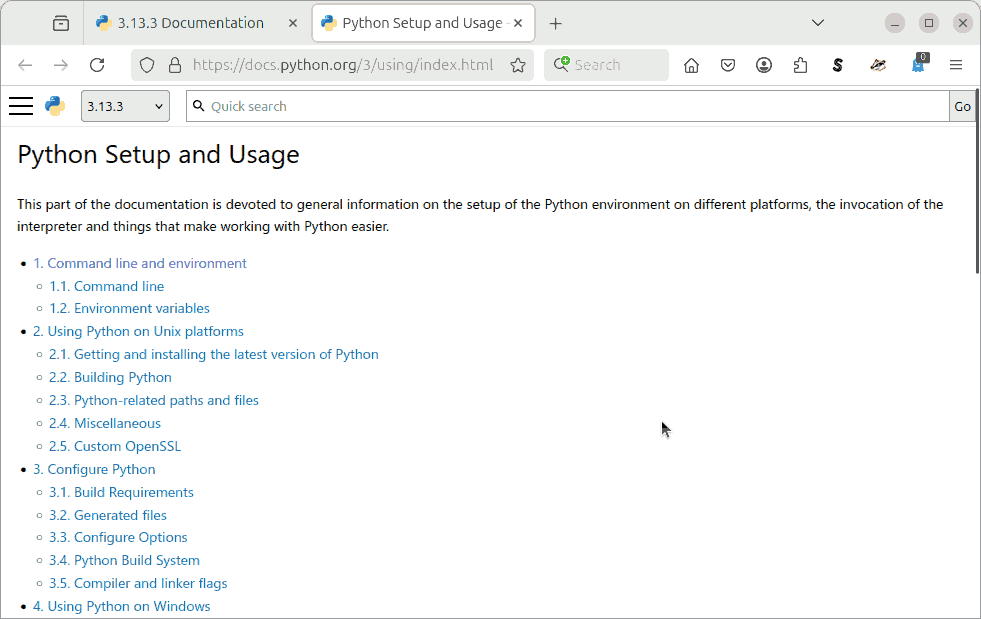
\includegraphics[width=0.47\linewidth]{\currentDir/pythondocOther01setupAndUsage}}}%
%
\floatSep%
%
\subfloat[][%
The \citetitle{PSF:P3D:TPT} page~\cite{PSF:P3D:TPT} page at~\citeurl{PSF:P3D:TPT}.%
\label{fig:pythondocOther02tutorial}%
]{\tightbox{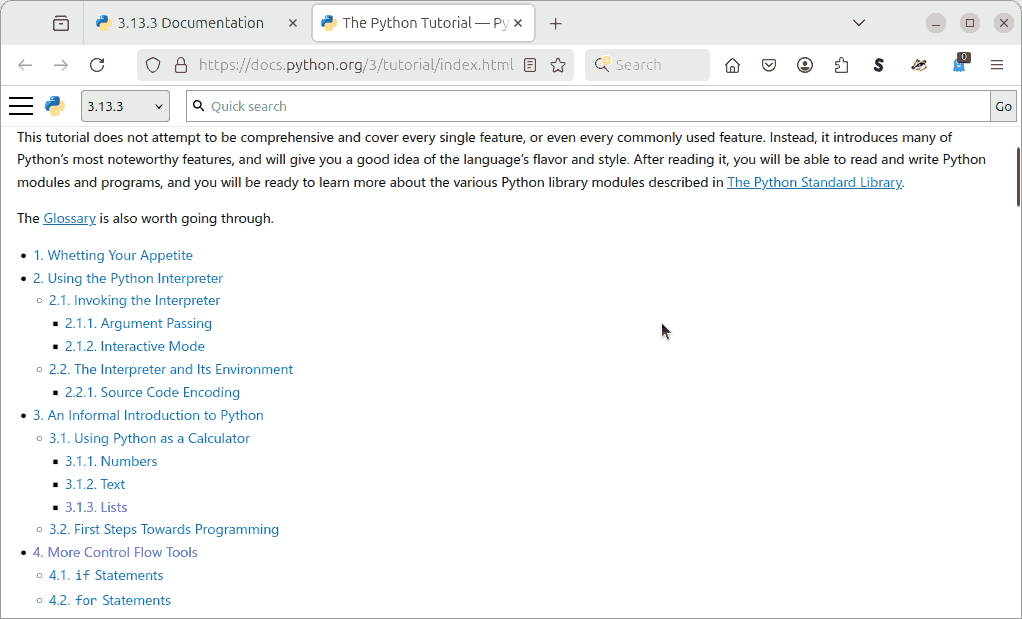
\includegraphics[width=0.47\linewidth]{\currentDir/pythondocOther02tutorial}}}%
%
\floatRowSep%
%
\subfloat[][%
The \citetitle{PSF:P3D:TPSL} page~\cite{PSF:P3D:TPSL} at~\citeurl{PSF:P3D:TPSL}.%
\label{fig:pythondocOther03standardLibrary}%
]{\tightbox{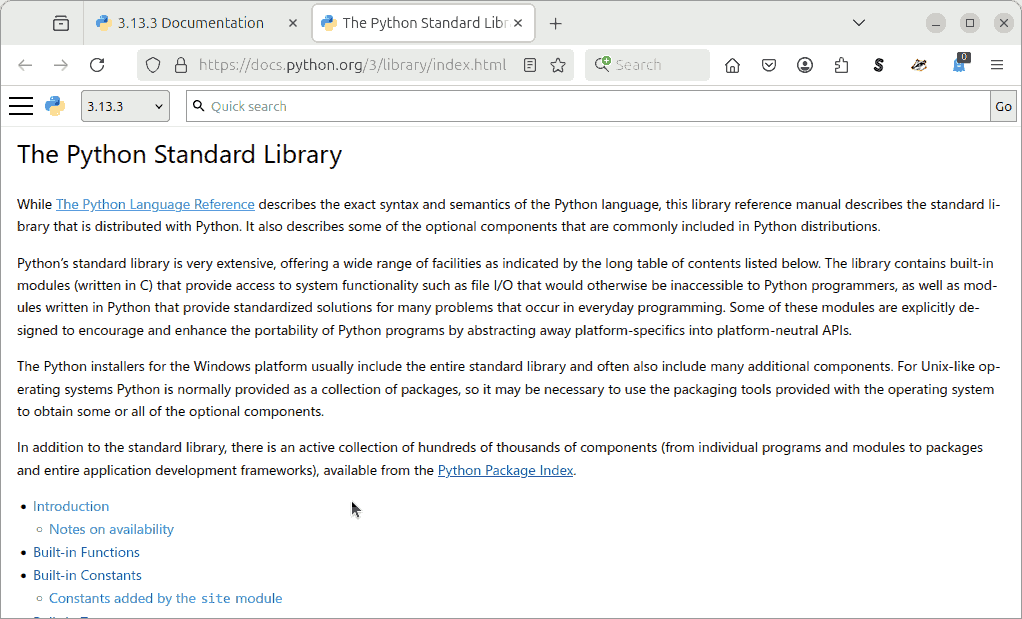
\includegraphics[width=0.47\linewidth]{\currentDir/pythondocOther03standardLibrary}}}%
%
\floatSep%
%
\subfloat[][%
The \citetitle{PEP0} page~\cite{PEP0} at~\citeurl{PEP0}.%
\label{fig:pythondocOther04pep0}%
]{\tightbox{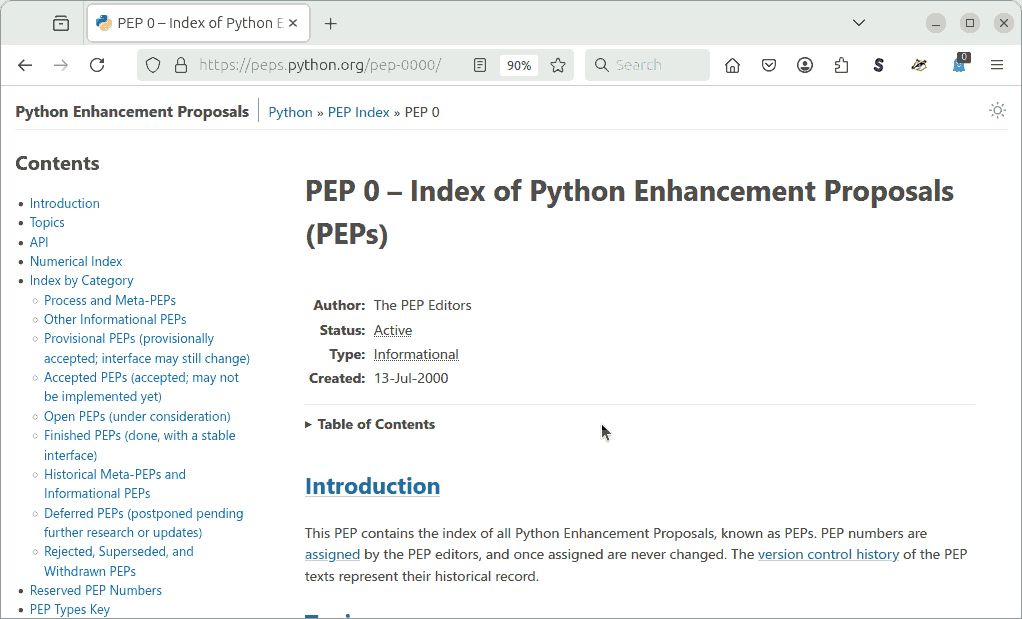
\includegraphics[width=0.47\linewidth]{\currentDir/pythondocOther04pep0}}}%
%
\caption{Several important authoritative online resources on \python.}%
\label{fig:pythondoc:D}%
\end{figure}%
%
Before getting to the end of this section, let us also note:
Besides being a source of authoritative information about \python, the official website \citeurl{PSF:P3D} also offers a variety of other useful information.
You may have already used the \citetitle{PSF:P3D:PSAU} page~\cite{PSF:P3D:PSAU} at~\citeurl{PSF:P3D:PSAU}, screenshotted in \cref{fig:pythondocOther01setupAndUsage}, when installing \python\ on your system.

The \citetitle{PSF:P3D:TPT} page~\cite{PSF:P3D:TPT} page at~\citeurl{PSF:P3D:TPT} and shown in \cref{fig:pythondocOther02tutorial} offers several useful tutorials.
Actually, it describes many of the techniques that we discuss in this book in much depth and very nicely, probably even better than this book.
I very strongly urge you to also read this website.

The \citetitle{PSF:P3D:TPSL} page~\cite{PSF:P3D:TPSL} at~\citeurl{PSF:P3D:TPSL} depicted in \cref{fig:pythondocOther03standardLibrary} contains the specification of all the standard functions that ship with \python.
It is therefore a very useful tool when checking what a function \emph{actually} does, to complement our learned knowledge.

Finally, the \citetitle{PEP0} page~\cite{PEP0} at~\citeurl{PEP0} shown in \cref{fig:pythondocOther04pep0} contains all changes and additions to the \python\ language since roughly the year~2000.
We can find many of the language utilities that we are using in this book defined in a so-called~\emph{Python Enhancement Proposal~(PEP)}.%
%
\endhsection%
%
\hsection{Summary}%
So what did we learn in this section?
We learned that an important tool for a programmer is the official documentation of the programming language that they are using and of the tools that they employ.
We can trust the documentation.
It is an important skill to be able to sit down, concentrate, and read such documentation.
If you have a certain question or task, it is very useful if you are able to work your way through a large body of text, be it some documentation or some standard, to identify which information is relevant for your situation, to ingest and understand this information, and to determine the actions you need to take to bring the task to a successful end.

That being said, it is not always possible to easily find the information that you are looking for in the documentation.
Luckily, there exist other useful tools that you can apply.
You can use search engines, you can read in internet forums like \citetitle{SE:SO}~\cite{SE:SO}, and you can ask your questions to an~\pgls{AI}.
All of these tools can guide you to the right answer.
We always need to check these answers by circling back to the authoritative documentation, because there is no guarantee that the answeres are correct or up-to-date.

All non-authoritative sources provide answers that, ultimately, are grounded on prior human experience and training.
On one hand, humans can make errors and not even know that they made them.
on the other hand, non-authoritative sources might be outdated.

There are two (known) differences between \pgls{AI} tools and human-written sources, though.
First, \pgls{AI} tools can make errors that no human would make.
An illustrative example in the \python\ world is given in~\cite{BSHETB:VSK2025CIC}, where it is documented that Microsoft Copilot renamed a class in a misleading way, leading to a particularly hard-to-find error.
Second, sometimes, an \pgls{AI} may reference non-existing packages~\cite{AT:G2025AGCCBADFTSSCHW}.
Therefore, once you found an answer to your question, you need to take the new information and check it with the documentation.

Anyway, as example for searching information using \pgls{AI} tools, we looked for a function that rounds floating point numbers towards positive infinity.
We did not know what this function was called~(or whether it even exists).
The \pgls{AI} told us that it was called \pythonilIdx{ceil}.
We got the exact same information by using a search engine and by using a community portal.
Regardless how we got that information, we would not just use the function \pythonilIdx{ceil} in our code directly.
We would go back to the official \python\ documentation and search for \pythonilIdx{ceil}.
Only after checking the documentation, we would have clarity and confidence that we will produce the right code.%
\endhsection%
%
\FloatBarrier%
\endhsection%
%
